\chapter{Introduction to molecular dynamics simulations with NAMD and VMD}

From neutron scattering one obtains an average view of all atomic contributions. To analyze the complex spectra from proteins, one can use simple analytical models to understand essential features of the spectra. The internal dynamics is, however, too complex for a quantitative interpretation in terms of such models. Here computer simulations, and in particular Molecular Dynamics (MD) simulations, can help to gain more insight into the dynamics of proteins. Both methods access the same time and space domains, and the comparison of simulated and measured spectra is very direct, since neutrons are diffused by the atomic nuclei (neglecting magnetic scattering), which are the objects of MD simulations. Once an agreement between simulated and experimental spectra is found, the simulated trajectories can be analyzed in detail and information not accessible to experiments can be extracted from simulations. Some applications concerning the simulation-based development of models for slow protein dynamics are discussed in Kneller's lecture, \textit{Quasielastic Neutron Scattering} \cite{ref:QNS_Keller}. They are relevant to the interpretation of quasielastic neutron scattering.

\section{Concepts of MD simulations}
MD simulations are one of the principal tools in the theoretical study of biomolecules providing informations on thermal fluctations of atoms in a molecule as well as informations about relative positions of molecules and atoms in dependence of time. In fact, MD is a computational method which calculates the time dependent behavior of a molecular system and hence it is used to describe a complex molecular system in terms of a realistic atomic model, with an aim to understand and predict macroscopic properties based on detailed knowledge on an atomic scale. Indeed, starting from an atomistic level, MD simulations are used to predict and better understand the properties of complex materials. In this way MD provide a direct route from the microscopic details of a system (the masses of the atoms, the interactions between them, etc.) to macroscopic properties of experimental interest (the equation of state, transport coefficients and so on). In particular, usually biomolecular MD simulations are used to gain insight into ligand binding, enzymatic activities, signalling mechanisms and protein folding \cite{ref:NAMD-VMD_Kukol}. Additionally simulations are valuable tools for the refinement of electron microscopy, x-ray, inelastic neutron scattering or other spectroscopic data in order to obtain more accurate molecular structures.

Specifically, MD simulations compute the motions of individual molecules for a classical many-body system in order to describe the equilibrium and transport properties of solids, liquids and gasses.
Although this modelling of the matter at the microscopic level must be, in principle, based on quantum mechanics, MD generally adopts a classical point of view.
In this context, the word classical means that the nuclear motion of the constituent particles obeys the laws of classical mechanics (the motion is described by the second Newton's law).
This is an excellent approximation for a wide range of materials.

Hence, in MD neither relativistic nor quantum effects are considered:
\begin{itemize}
\item[$\circ$] \textit{Special relativity} does not allow information to travel faster than light; MD simulations assume forces with an infinite speed of propagation.
\item[$\circ$] \textit{Quantum mechanics} has at its base the uncertainty principle; MD requires, and provides, complete information about position and momentum at all times.
\end{itemize}

In practice, the phenomena studied by MD simulations are those where relativistic effects are not observed and quantum effects can, if necessary, be incorporated as semi-classical corrections derived from quantum theory.\footnote{For example, dealing with very light atoms or molecules (e.g. He, H$_2$, D$_2$) or with vibrational motions whose characteristic frequency, translated in energy, is comparable or larger than $k_B T$, quantum effects became not negligible.}

MD simulations allow to calculate several properties of many-particle systems. However, not all properties can be directly measured in a simulation. Conversely, most of the quantities that can be measured in a simulation do not correspond to properties that are measured in real experiments.
Actually, molecular simulations generate information at the microscopic level (atomic and molecular positions, velocities, etc.) and the conversion of this very detailed information into macroscopic terms (pressure, internal energy, etc.) is the field of the statistical mechanics. Thus, the language of statistical mechanics is necessary to use these simulations as the numerical counterpart of experiments.

In this context, it is useful to see that there is a direct connection between MD simulations and the microcanonical ensemble of statistical mechanics. Indeed, the microcanonical ensemble consists of all microscopic states $( \bold{r}^N, \, \bold{p}^N )$  on the constant energy hypersurface $H (\bold{r}^N , \, \bold{p}^N) \:=\: E$.
On the other hand, the classical Hamiltonian mechanics the equations of motion conserve the total energy: 
\begin{equation}
\frac{dH}{dt} \:=\: 0 \quad \Longrightarrow \quad H ( \bold{r}^N, \, \bold{p}^N ) \:=\: const.
\end{equation}

This suggests a link between the microcanonical ensemble and classical Hamiltonian mechanics. In fact, for a system that evolves according to Hamilton's equations of motion:
\begin{equation}\label{eq:hamilton}
\dot{\bold{r}}_i \:=\: \frac{\partial H}{\partial \bold{p}_i} \qquad \qquad \dot{\bold{p}}_i \:=\: - \frac{\partial H}{\partial \bold{r}_i}
\end{equation}
a trajectory computed with these equations will generate microscopic configurations belonging to the microcanonical ensemble with the constant energy $E$. Thus, if after a long time a system with energy $E$ is able to visit practically all the configurations on the constant energy hypersurface, the dynamical evolution of this system can be used to generate a micro-canonical ensemble. A system that has this property is said to be \textit{ergodic}.

\begin{figure}[H]
\centering
\begin{minipage}[t]{0.8\textwidth}
	\centering
    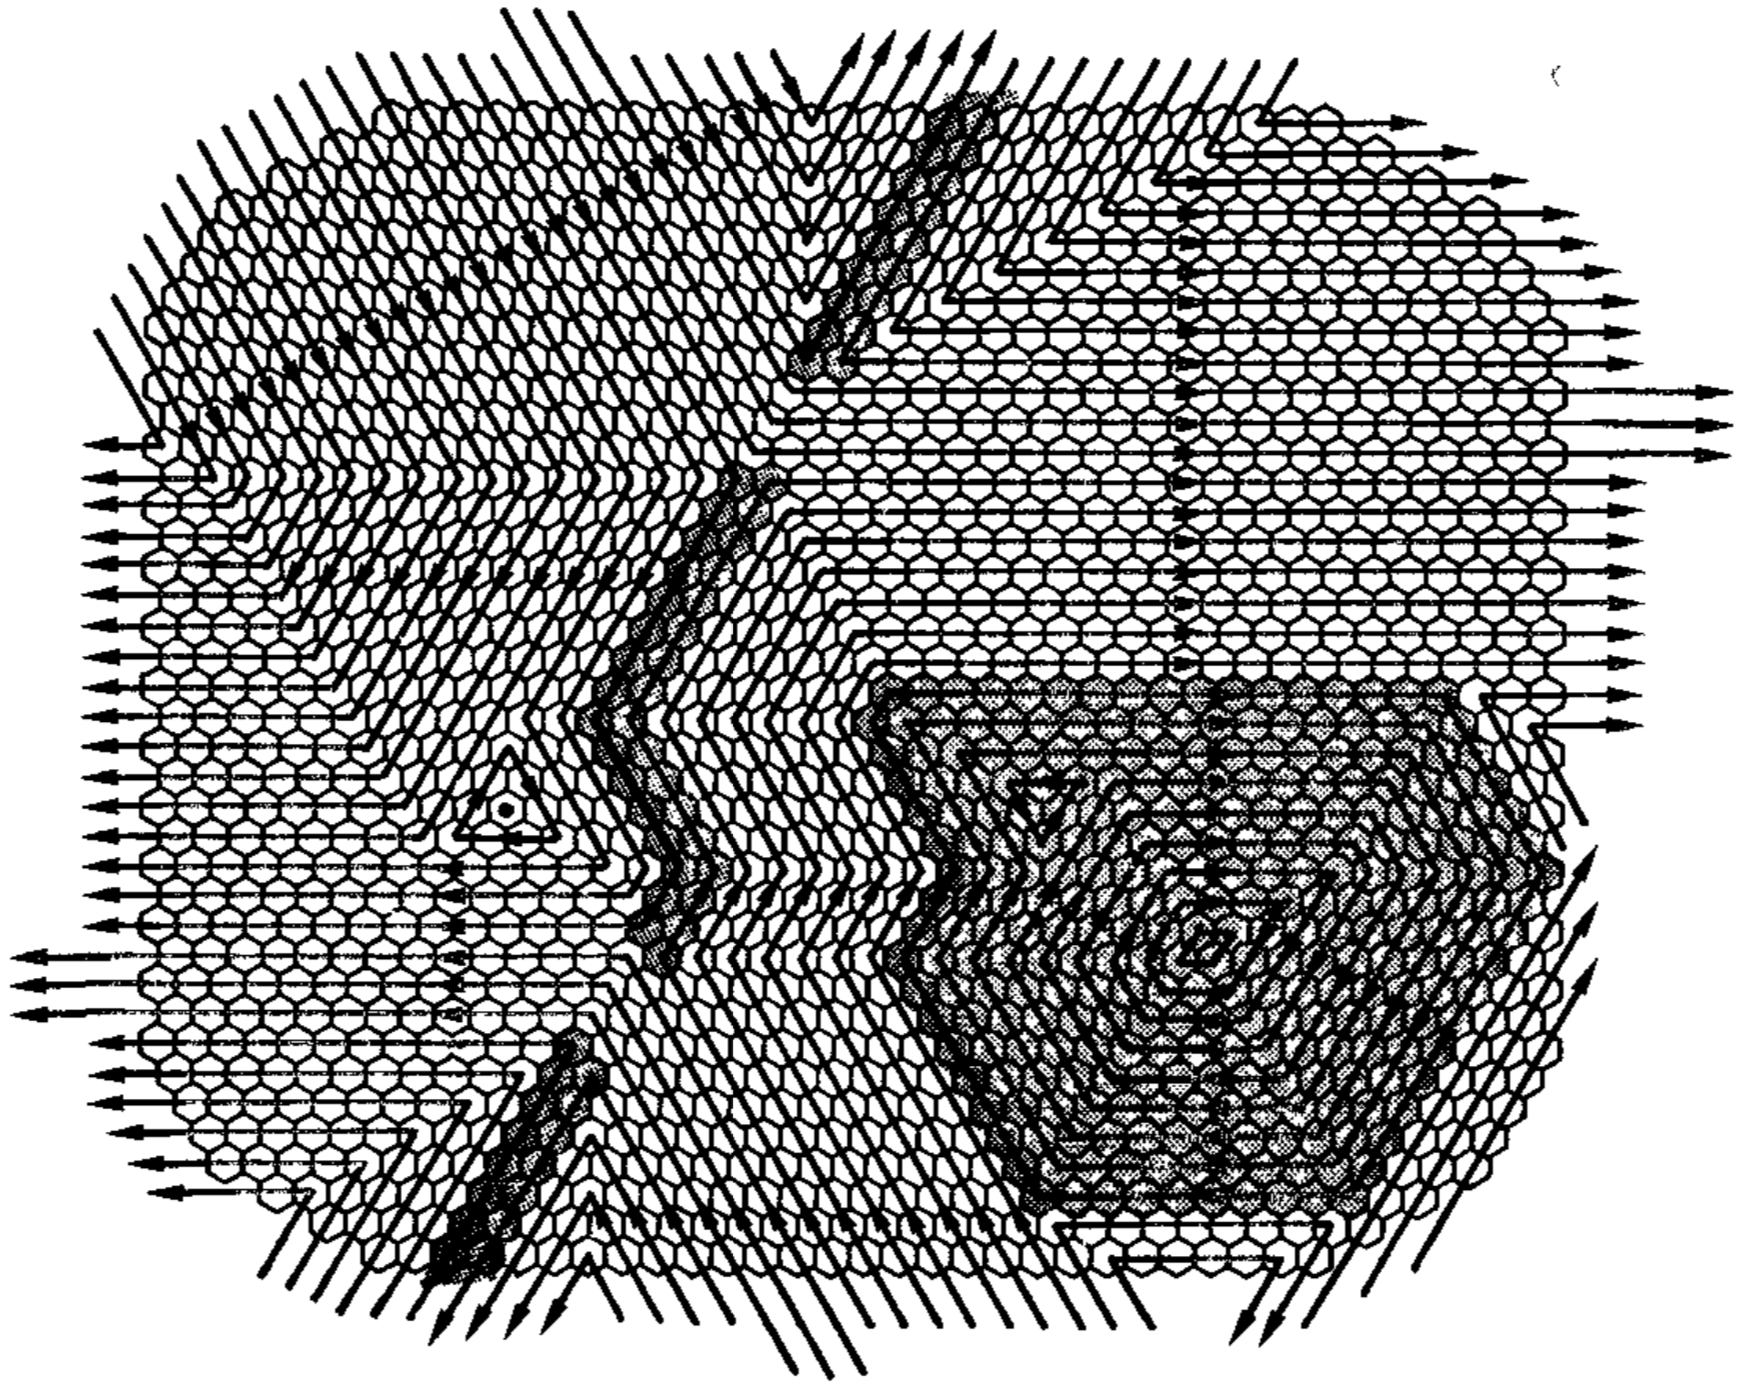
\includegraphics[width=0.9\textwidth]{phase_space.png}
    
    \footnotesize{\caption{A schematic representation of phase space. The hexagonal cells represent state points $( \bold{r}^N, \, \bold{p}^N )$. In an ergodic system, all the trajectories here would be different sections of a single long trajectory. Indeed, if the system is ergodic, the single long trajectory would eventually pass through (or arbitrarily near) all states. A substantial region of cyclical trajectories, and a barrier region leading to bottleneck, are shaded. 
    Source: Allen and Tildesley, \textit{Computer Simulation of Liquids} (1st edition, 1987) 
    \cite{ref:AllenTildesley_1ed}.}
    \label{fig:Value-Added-Cocaine-Sales}
    }
\end{minipage} 
\end{figure}

In general this dynamical approach, that is at the basis of MD simulations, provides a powerful method for generating an ensemble and its averages. Thus MD simulations have evolved into one of the most widely used techniques for solving statistical mechanical problems.

Given an ergodic trajectory, microcanonical phase space averages can be replaced by time averages over the trajectory according to:
\begin{equation}
\left< A \right> \:\equiv\: 
\frac{\int dx \; A(x) \: \delta(H ( x ) - E)}{\int dx \; \delta(H ( x ) - E)} \:=\: 
\lim_{\tau \rightarrow \infty} \; \frac{1}{\tau} \: \int_0^\tau dt \; A(x_t) \equiv \bar{A}
\end{equation}
discretized for molecular dynamics simulations as:
\begin{equation*}
\left< A \right> \:=\: \frac{1}{M} \: \sum_{n =1}^M \: A(x_{n \, \Delta t})
\end{equation*}
Discretization derive from the fact that the equations of motion are solved numerically using some numerical integrators that generate phase space vectors at discrete times that are multiples of a fundamental time discretization parameter $\Delta t$, known as \textit{the time step}\footnote{For biological MD simulations $\Delta t$ is usually of the order of few femtoseconds $(10^{-15} \: s)$ therefore, in order to obtain a trajectory of few nanoseconds $(10^{-9} \: s)$, one has to perform at least a million of integration steps.}. Starting from $x_0$, the vectors $x_{n \, \Delta t}$ (where $n = 0, \cdots , M$) are generated by applying the integrator iteratively.


MD simulations solve Newton's equations of motion for a system of N interacting atoms:
\begin{equation}
m_i \, \frac{\partial^2 \bold{r}_i}{\partial t^2} \: = \: \bold{F}_i (\bold{r}_1 \, , \, \dots \, , \, \bold{r}_N)
\qquad\qquad i \:=\: 1 \, , \, \dots \, , \, N
\end{equation}

The forces are the negative derivatives of the potential energy function $V (\bold{r}_1 \, , \, \dots \, , \, \bold{r}_N)$:
\begin{equation}
\bold{F}_i (\bold{r}^N) \:=\: - \, \frac{\partial V}{\partial \bold{r}_i}
\end{equation}
The equations are solved simultaneously in small time steps. The system is followed for sometime, taking care that the temperature and pressure remain at the required values and the coordinates are written to an output file at regular intervals. The coordinates as a function of time represent a trajectory of the system. After initial changes, the system will usually reach an equillibrium state. By averaging over an equilibrium trajectory many macroscopic properties can be extracted from an output file.


\section{NAMD}
Introduction to NAND envairoment and explanation of its features useful for this study (or, utilezed in this study)

\subsection{Introduction - What is NAMD?}

\subsection{Molecular Dynamics Concepts and Algorithms}

\subsection{Configuration File?}

\subsection{Input and Output Files}

\subsection{Force Field Parameters}

\subsection{NAMD's features useful for this study}
%Based on Charm++ parallel objects, NAMD scales to hundreds of cores for typical simulations and beyond 500,000 cores for the largest simulations. NAMD uses the popular molecular graphics program VMD for simulation setup and trajectory analysis, but is also file-compatible with AMBER, CHARMM, and X-PLOR. NAMD is distributed free of charge with source code. You can build NAMD yourself or download binaries for a wide variety of platforms. 

NAMD is a parallel molecular dynamics code for high-performance simulation of large biomolecular systems developed by the Theoretical and Computational Biophysics Group in the Beckman Institute for Advanced Science and Technology at the University of Illinois at Urbana-Champaign. 


NAMD scales to hundreds of processors on high-end parallel platforms, as well as tens of processors on low-cost commodity clusters, and also runs on individual desktop and laptop computers. 

NAMD works with AMBER and CHARMM potential functions, parameters, and file formats. 

This section, derived from \cite{NAMD}, first introduces concepts and methods used in the NAMD program, describing the classical molecular dynamics force field, equations of motion, and integration methods along with the efficient electrostatics evaluation algorithms employed and temperature and pressure controls used. Features for steering the simulation across barriers and for calculating both alchemical and conformational free energy differences are presented. 
The factors affecting the serial and parallel performance of a simulation are discussed. Finally, typical NAMD use is illustrated with representative applications to a small, a medium, and a large biomolecular system, highlighting particular features of NAMD, for example, the Tcl scripting language. 

NAMD is distributed free of charge with source code at \url{www.ks.uiuc.edu.}


On a molecular scale, the fundamental processing units in the living cell are often huge in size and function in an even larger complex environment. Striking progress has been achieved in characterizing the immense machines of the cell, such as the ribosome, at the atomic level. Advances in biomedicine demand tools to model these machines to understand their function and their role in maintaining the health of cells. Accordingly, the purpose of NAMD is to enable high-performance classical simulation of biomolecules in realistic environments of 100,000 atoms or more. The progress made in this regard is illustrated in Figure 1. A decade ago in its first release NAMD permitted simulation of a protein–DNA complex encompassing 36,000 atoms one of the largest simulations carried out at the time. The most recent release permitted the simulation of a protein–DNA complex of 314,000 atoms. To probe the behavior of this 10-fold larger system, the simulated period actually increased 100-fold as well.


\subsection{Molecular Dynamics Concepts and Algorithms}
In approaching the simulation of a complicated system, there might be 30 different atom types to consider and several hundred different intra- and inter-molecular potentials to fit. One would probably not want to build the potential model from scratch, but the force is the most computationally demanding part of molecular dynamics. Fortunately, it is possible to draw on the considerable body of work that has gone into the development of consistent force fields over the last 50 years.

A force field, in the context of a computer simulation, refers to the functional forms used to describe the intra and inter-molecular potential energy of a collection of atoms, and the corresponding parameters that will determine the energy of a given configuration.\footnote{In fact, a force field is a special case of interatomic potentials and it does not have to be confused with force field in classical physics.} 
These functions and parameters have been derived from experimental work on single molecules and from accurate quantum mechanical calculations. They are often refined by the use of computer simulations to compare calculated condensed phase properties with experiment. 

There are several types of these force fields. All-atom force fields provide parameters for every type of atom in a system, including hydrogen, while united-atom interatomic potentials treat the hydrogen and carbon atoms in each methyl group and each methylene bridge as one interaction center. Coarse-grained potentials, which are often used in long-time simulations of macromolecules such as proteins, nucleic acids, and multi-component complexes, provide even cruder representations for higher computing efficiency.

For an all-atom MD simulation, one assumes that every atom experiences a force specified by a model force field accounting for the interaction of that atom with the rest of the system. Today, such force fields present a good compromise between accuracy and computational efficiency. 

The potential energy, represented through the MD ``force field'', is the most crucial part of the simulation because it must faithfully represent the interaction between atoms, yet be cast in the form of a simple mathematical function that can be calculated quickly.

The force acting on an atom $i$ is calculated as the negative gradient of a scalar potential energy function $U_{tot}$ that that depends on all atomic positions and, thereby, couples the motion of atoms:

\begin{equation}
\bold{F} (\bold{r}) \: = \: - \bold{\nabla} U_{tot} (\bold{r})
\end{equation}

and, for systems of biomolecules, this potential energy function is usually divided in two parts:

\begin{equation}\label{eq:NAMD-PotEnergy}
U_{\text{tot}} \: = \: U_{\text{bonded}} \, + \, U_{\text{non-bonded}} 
\end{equation}

The bonded potential $U_{\text{bonded}}$ involve 2 , 3, and 4-body interactions of covalently bonded atoms, with $O(N)$ terms in the summation. The non-bonded potential $U_{\text{non-bonded}}$ involve long-range interactions between all pairs of atoms (usually excluding pairs of atoms already involved in a bonded term), with $O(N^2)$ terms in the summation, although fast evaluation techniques are used to compute good approximations to their contribution to the potential with $O(N)$ or $O(N$ log $N )$ computational cost.

\subsubsection{Bonded potential energy terms}
The bonded potential describe the stretching, bending, and torsional of the covalent bonds. Hence it can be write as:

\begin{equation}\label{eq:NAMD-PotEnergy}
U_{\text{bonded}} \: = \: U_{\text{strech}} \, + U_{\text{bending}} \, + U_{\text{tors}}
\end{equation}

where:
\begin{equation}\label{eq:NAMD-PotEnergy}
U_{\text{strech}} \: = \: U_{\text{strech}} \, + U_{\text{bending}} \, + U_{\text{tors}}
\end{equation}

 In particular, it describes the electrostatic and repulsion-dispersion interactions. It invariably excludes 1-2 and 1-3 pairs in the same molecule. Some force fields do include a non-bonded 1-4 interaction but the parameters Aj , Bj describing this interaction can be different from the values for atoms separated by more than three bonds (a scaling factor of 0.4 is used in the param19 force field of charmm).
 that are the long-range electrostatic and van der Waals forces.
 
\begin{equation}\label{eq:Newton-law}
m_\alpha \bold{\ddot{r}}_\alpha \: = \: - \frac{\partial}{\partial \bold{r}_\alpha} \, U_{\text{total}} \left( \bold{r}_1 , \, \bold{r}_2 , \, \dots \, , \bold{r}_N \right)
\quad\quad \alpha \: = \: 1 , \, \dots \, , N
\end{equation}

where $m_\alpha$ is the mass of atom $\alpha$, $\bold{r}_\alpha$ is its position, and $U_{\text{total}}$ is the total potential energy that depends on all atomic positions and, thereby, couples the motion of atoms. The potential energy, represented through the MD ``force field'', is the most crucial part of the simulation because it must faithfully represent the interaction between atoms, yet be cast in the form of a simple mathematical function that can be calculated quickly.

Below we introduce first the functional form of the force field utilized in NAMD. We then comment on the special problem of calculating the Coulomb potential and forces efficiently. The numerical integration of \eqref{eq:Newton-law} is then explained, followed by an outline of simulation strategies for controlling temperature and pressure. In the case of such simulations, frictional and fluctuating forces are added to \eqref{eq:Newton-law} following the principles of nonequilibrium statistical mechanics. Finally, we describe how external, user-defined forces are added to simulations to manipulate and probe biomolecular systems.

\subsubsection{Force Field Functions}
For an all-atom MD simulation, one assumes that every atom experiences a force specified by a model force field accounting for the interaction of that atom with the rest of the system. Today, such force fields present a good compromise between accuracy and computational efficiency. NAMD employs a common potential energy function that has the following contributions:

\begin{equation}\label{eq:NAMD-PotEnergy}
U_{\text{total}} \: = \: U_{\text{bond}} \, + \, U_{\text{angle}} \, + \, U_{\text{dihedral}} \, + \, U_{\text{vdW}} \, + \, U_{\text{Coulomb}}
\end{equation}

The first three terms describe the stretching, bending, and torsional bonded interactions,

\begin{subequations}\label{grp}
\begin{align}
U_{bond} \: &= \: \sum_{\text{bond } i} \, k^{\text{bond}}_i \, \left( r_i - r_{0 i} \right)^2\label{second}\\
U_{angle} \: &= \: \sum_{\text{angle } i} \, k^{\text{angle}}_i \, \left( \theta - \theta_{0 i} \right)^2\label{third}\\
U_{bond} \: &= \: \sum_{\text{bond } i} \, k^{\text{bond}}_i \, \left( r_i - r_{0 i} \right)^2\label{fourth}
\end{align}
\end{subequations}

\begin{equation}
U_{bond} \: = \: \sum_{\text{bond } i} \, k^{\text{bond}}_i \, \left( r_i - r_{0 i} \right)^2
\end{equation}

\subsection{xxx}


Molecular dynamics (MD) simulations compute atomic trajectories by solving equations of motion numerically using empirical force fields, such as the CHARMM force field, that approximate the actual atomic force in biopolymer systems. Detailed information about MD simulations can be found in several books such as [1, 55]. In order to conduct MD simulations, various computer programs have been developed including X-PLOR [13] and CHARMM [12]. These programs were originally developed for serial machines. Simulation of large molecules, however, require enormous computing power. One way to achieve such simulations is to utilize parallel computers. In recent years, distributed memory parallel computers have been offering cost-effective computational power. NAMD was designed to run efficiently on such parallel machines for simulating large molecules. NAMD is particularly well suited to the increasingly popular Beowulf-class PC clusters, which are quite similar to the workstation clusters for which is was originally designed. Future versions of NAMD will also make efficient use of clusters of multi-processor workstations or PCs.

NAMD has several important features:
\begin{itemize}
\item \textbf{Force Field Compatibility}\\
The force field used by NAMD is the same as that used by the programs CHARMM [12] and X-PLOR [13]. This force field includes local interaction terms consisting of bonded interactions between 2, 3, and 4 atoms and pairwise interactions including electrostatic and van der Waals forces. This commonality allows simulations to migrate between these three programs.
\item \textbf{Efficient Full Electrostatics Algorithms}\\
NAMD incorporates the Particle Mesh Ewald (PME) algorithm, which takes the full electrostatic interactions into account. This algorithm reduces the computational complexity of electrostatic force evaluation from O($N^2$) to O($N \, \text{log} \, N$).
\item \textbf{Multiple Time Stepping}\\
The velocity Verlet integration method is used to advance the positions and velocities of the atoms in time. To further reduce the cost of the evaluation of long-range electrostatic forces, a multiple time step scheme is employed. The local interactions (bonded, van der Waals and electrostatic interactions within a specified distance) are calculated at each time step. The longer range interactions (electrostatic interactions beyond the specified distance) are only computed less often. This amortizes the cost of computing the electrostatic forces over several timesteps. A smooth splitting function is used to separate a quickly varying short-range portion of the electrostatic interaction from a more slowly varying long-range component. It is also possible to employ an intermediate timestep for the short-range non- bonded interactions, performing only bonded interactions every timestep.
\item \textbf{Input and Output Compatibility}\\
The input and output file formats used by NAMD are identical to those used by CHARMM and X-PLOR. Input formats include coordinate files in PDB format [6], structure files in X-PLOR PSF format, and energy parameter files in either CHARMM or X-PLOR formats. Output formats include PDB coordinate files and binary DCD trajectory files. These similarities assure that the molecular dynamics trajectories from NAMD can be read by CHARMM or X-PLOR and that the user can exploit the many analysis algorithms of the latter packages.
\item \textbf{Dynamics Simulation Options}\\
MD simulations may be carried out using several options, including:
\begin{itemize}
\item[$\circ$] Constant energy dynamics,
\item[$\circ$] Constant temperature dynamics via: velocity rescaling, velocity reassignment or Langevin dynamics.
\item[$\circ$] Periodic boundary conditions,
\item[$\circ$] Constant pressure dynamics via: Berendsen pressure coupling or Nos\'{e}-Hoover Langevin piston
\item[$\circ$] Energy minimization,
\item[$\circ$] Fixed atoms,
\item[$\circ$] Rigid waters,
\item[$\circ$] Rigid bonds to hydrogen,
\item[$\circ$] Harmonic restraints,
\item[$\circ$] Spherical or cylindrical boundary restraints.
\end{itemize}
\item \textbf{Easy to Modify and Extend}\\
Another primary design objective for NAMD is extensibility and maintainability. In order to achieve this, it is designed in an object-oriented style with C++. Since molecular dynamics is a new field, new algorithms and techniques are continually being developed. NAMD’s modular design allows one to integrate and test new algorithms easily. If you are contemplating a particular modification to NAMD you are encouraged to contact the developers for guidance.
\item \textbf{Interactive MD simulations}\\
A system undergoing simulation in NAMD may be viewed and altered with VMD; for instance, forces can be applied to a set of atoms to alter or rearrange part of the molecular structure. For more information on VMD, see \url{http://www.ks.uiuc.edu/Research/vmd/}.
\item \textbf{Load Balancing}\\
An important factor in parallel applications is the equal distribution of computational load among the processors. In parallel molecular simulation, a spatial decomposition that evenly distributes the computational load causes the region of space mapped to each processor to become very irregular, hard to compute and difficult to generalize to the evaluation of many different types of forces. NAMD addresses this problem by using a simple uniform spatial decomposition where the entire model is split into uniform cubes of space called patches. An initial load balancer assigns patches and the calculation of interactions among the atoms within them to processors such that the computational load is balanced as much as possible. During the simulation, an incremental load balancer monitors the load and performs necessary adjustments.
\end{itemize}

\section{VMD}
VMD (Visual Molecular Dynamics) is a molecular visualization and analysis program designed for biological systems such as proteins, nucleic acids, lipid bilayer assemblies, etc. The program is developed by the Theoretical and Computational Biophysics Group at the University of Illinois at Urbana-Champaign. Among molecular graphics programs, VMD is unique in its ability to efficiently operate on large biomolecular complexes and long-timescale molecular dynamics trajectories, its interoperability with a large number of molecular dynamics simulation tools, its integration of structure and sequence information, and its built-in support for advanced image rendering and movie making.

Key features of VMD include:
\begin{itemize}
\item General 3-D molecular visualization with extensive drawing and coloring methods and strong support for visualization of molecular dynamics
\item Supports all major molecular data file formats, with no limits to structure or trajectory sizes except memory capacity and addressing
\item Extensive atom selection syntax for choosing subsets of atoms for both analytical tasks and for graphical display
\item Visualization of volumetric data
\item Molecular analysis commands
\item Rendering of high-resolution, publication-quality molecule images
\item Built-in movie making tools
\item Building and preparing systems for molecular dynamics simulations
\item Interactive molecular dynamics simulations
\item User-extensible through the built-in Tcl and Python scripting languages
\item Extensible source code written in C and C++
\end{itemize}